\documentclass[oneside, 11pt]{article}

\usepackage[T1]{fontenc}
\usepackage[utf8]{inputenc}
\usepackage[dutch]{babel}

\usepackage{fouriernc}
\usepackage[detect-all, load-configurations=binary,
            separate-uncertainty=true, per-mode=symbol,
            retain-explicit-plus, range-phrase={ tot }]{siunitx}

\usepackage{setspace}
\setstretch{1.2}

\setlength{\parskip}{\smallskipamount}
\setlength{\parindent}{0pt}

\usepackage{geometry}
\geometry{marginparwidth=0.5cm, verbose, a4paper, tmargin=3cm, bmargin=3cm, lmargin=2cm, rmargin=2cm}

\usepackage{float}

\usepackage[fleqn]{amsmath}
\numberwithin{equation}{section}
\numberwithin{figure}{section}

\usepackage{graphicx}
\graphicspath{{Figures/}}
\usepackage{subfig}

\usepackage{tikz}
\usetikzlibrary{plotmarks}

\usepackage{fancyhdr}
\pagestyle{fancy}
\fancyhf{}
\rhead{\thepage}
\renewcommand{\footrulewidth}{0pt}
\renewcommand{\headrulewidth}{0pt}

\usepackage{relsize}
\usepackage{xspace}
\usepackage{url}

\newcommand{\figref}[1]{Figuur~\ref{#1}}

\newcommand{\hisparc}{\textsmaller{HiSPARC}\xspace}
\newcommand{\kascade}{\textsmaller{KASCADE}\xspace}
\newcommand{\sapphire}{\textsmaller{SAPPHiRE}\xspace}
\newcommand{\jsparc}{\textsmaller{jSparc}\xspace}
\newcommand{\hdf}{\textsmaller{HDF5}\xspace}
\newcommand{\aires}{\textsmaller{AIRES}\xspace}
\newcommand{\csv}{\textsmaller{CSV}\xspace}
\newcommand{\python}{\textsmaller{PYTHON}\xspace}
\newcommand{\corsika}{\textsmaller{CORSIKA}\xspace}
\newcommand{\labview}{\textsmaller{LabVIEW}\xspace}
\newcommand{\daq}{\textsmaller{DAQ}\xspace}
\newcommand{\adc}{\textsmaller{ADC}\xspace}
\newcommand{\adcs}{\textsmaller{ADC}s\xspace}
\newcommand{\Adcs}{A\textsmaller{DC}s\xspace}
\newcommand{\hi}{\textsc{h i}\xspace}
\newcommand{\hii}{\textsc{h ii}\xspace}
\newcommand{\mip}{\textsmaller{MIP}\xspace}
\newcommand{\hisparcii}{\textsmaller{HiSPARC II}\xspace}
\newcommand{\hisparciii}{\textsmaller{HiSPARC III}\xspace}
\newcommand{\pmt}{\textsmaller{PMT}\xspace}
\newcommand{\pmts}{\textsmaller{PMT}s\xspace}

\DeclareSIUnit{\electronvolt}{\ensuremath{\mathrm{e\!\!\:V}}}

\DeclareSIUnit{\unitsigma}{\ensuremath{\sigma}}
\DeclareSIUnit{\mip}{\textsmaller{MIP}}
\DeclareSIUnit{\adc}{\textsmaller{ADC}}

\DeclareSIUnit{\gauss}{G}
\DeclareSIUnit{\parsec}{pc}
\DeclareSIUnit{\year}{yr}


\usepackage{xfrac}
\usepackage{array}

\title{Stationsonderhoud}
\author{C.G.N. van Veen}
\docrecept{1}{SO}
\version{1.0}

\begin{document}

\maketitle

\begin{tabular}{|>{\raggedright}p{3cm}|>{\raggedright}p{12cm}|}
\hline
leerjaar & niveau \tabularnewline
\hline
5/6 VWO & beginnend \tabularnewline
\hline
\end{tabular}

\section{lesmateriaal}

Dit recept voor werken met \hisparc gaat in op het onderhoud van een \hisparc station.
Leerlingen krijgen eerst een introductie over kosmische straling en gaan
dan aan de slag met het analyseren van een \hisparc station en
uiteindelijk stellen de leerlingen het station optimaal in.

\textbf{Alles wat nodig is voor deze lessenserie vindt u hier:}
\url{http://docs.hisparc.nl/zips/onderhoud_station.zip}


\textit{Opmerking:} leerlingen hebben bij deze lessenserie baat bij kennis van
elektrische velden, versnelspanning, energie van fotonen, radioactief verval,
deeltjesfysica en de Lorentzfactor ($\gamma$):
\begin{equation}
    E = h \cdot f
\end{equation}
\begin{equation}
    q \cdot {U_{AK}} = \sfrac{1}{2} \cdot m \cdot {v^2}
\end{equation}
\begin{equation}
    \gamma = \frac{1}{\sqrt{1-\frac{v^2}{c^2}}}
\end{equation}


\begin{tabular}{|c|p{9cm}|c|}
\hline
lesnummer & lesdocument & bron \tabularnewline
\hline
1 & Terminologie, Cosmic air showers, Werkblad: cosmic air showers,
kosmische straling & Infopakket\tabularnewline
\hline
2 & Uitleg \hisparc en Controle station, Werkblad: detecteren & Infopakket, RouteNet\tabularnewline
\hline
3 & Inregelen PMT's, Werkblad : Fotomultiplier, Opdracht: instellen PMT's van station & Infopakket, RouteNet \tabularnewline
\hline
\end{tabular}


\section{Les 1}

Introductie van kosmische straling. In deze les starten we met
achtergrond materiaal en een werkblad. Tijdens deze les kunnen
leerlingen ook een station bezoeken als dat op school staat. Belangrijk
is dat er een introductie op kosmische straling gegeven wordt en dat de
terminologie duidelijk wordt gemaakt.
Behandel in ieder geval:

\begin{itemize}
    \item Wat is kosmische straling?
    \item Hoe ontstaat een deeltjeslawine?
    \item Hoe worden deze deeltjes in de lawine op aarde gedetecteerd?
\end{itemize}

\textbf{Opmerking:}
Van de \hisparc site (\url{www.hisparc.nl}) kunnen diverse bestaande powerpoint-presentaties
gedownload worden.
Deze presentaties mogen naar believen aangepast worden, om door leerlingen en docenten
in de klas te gebruiken.


\section{Les 2}

In deze les gaan we naar de meetstations van \hisparc kijken en met name naar de
afstelling van de detectoren en het onderhoud van een station.
We beginnen met achtergrondinformatie over de detectoren. In deze les is het
belangrijk dat in ieder geval pulshoogte-histogram uitgelegd wordt en hoe dit histogram
gemaakt wordt.

In deze les behandelen we zaken als:
\begin{itemize}
    \item Hoe meten de detectoren de deeltjes in de lawine?
    \item Wat is het pulshoogte-histogram?
    \item Hoe kunnen we foutmeldingen opsporen en oplossingen vinden?
\end{itemize}

In het document `controle station' wordt uitgelegd hoe leerlingen zelf
problemen met stations kunnen constateren en oplossen. Vooral meetproblemen, die te zien zijn in een
pulshoogte diagram, zie figuur 3.1 van document 'controle station' is
een probleem dat leerlingen zelf kunnen oplossen, dit leren ze ook in les 3.


\section{Les 3}

In deze les kijken we naar de DAQ software van het meetstation en gaan de leerlingen
zelf aan de slag met het instellen van de fotomultipliers (PMT's) van het station.
De leerlingen krijgen wat (meer) uitleg over de fotomultiplier en stellen via de \hisparc \daq
de juiste spanning in voor fotomultiplier.

In deze les behandelen we zaken als:
\begin{itemize}
    \item Hoe werkt een fotomultiplierbuis?
    \item Hoe kunnen we de spanning op de stations zo instellen dat er een
    goed pulshoogte diagram ontstaat?
\end{itemize}

In het document \textit{inregelen PMTs}, wordt een uitleg gegeven van de
werking van de fotomultiplier buis. In het document \textit{inregelen
PMTs} wordt naast de werking van de fotomultiplier ook de instelling van
de \hisparc \daq uitgelegd. Leerlingen kunnen dit gebruiken om de
instellingen van de PMT's van de detectoren van het \hisparc station aan
te passen en te verbeteren. De opdracht aan leerlingen is om het station perfect
in te stellen. D.w.z. dat de pieken van het pulshoogte- en pulsintegraalhistogram
over elkaar liggen na instelling.

\textbf{Korte handleiding van de opdracht: Instellen van het station} Hieronder staat een lijst van de handelingen.
Het verdient sterke aanbeveling om het hele document `inregelen PMT's' te lezen!

\begin{itemize}
    \item Zorg dat de \daq mode stopt. (dit betekent dat er geen data meer wordt verzonden.)
    \item Zorg dat je de adc alignment het gedaan, voor \hisparc III \daq wordt de common offset
    10
    \item Stel de spanning van de PMT in (vanaf 300 V beginnen!) Zie \figref{fig:PMT_instellen}.
    \item Test de spanning in het menu "statistics (trace\&trigger)", klik `start counting'.)
    \item De PMT is goed ingesteld op het moment, dat de `average per second (HIGH)'
    op ongeveer 120 komt en (LOW) rond de 250 uitkomt. Zie \figref{fig:instellen_PMT_values}.
    \item Pas de PMT spanning in kleine stapjes aan om deze waarden te verkrijgen. Klik na elke aanpassing op `save settings'
    \item Herhaal de meting tot dat de instellingen de juiste `average per second' hebben bereikt.
    \item De PMT zou nu juist ingesteld moeten zijn.
\end{itemize}


\section{Verdieping}

\begin{tabular}{|c|c|c|}
\hline
leerdoelen & beschrijving bron & bron \tabularnewline
\hline
Datareconstructie met \hisparc & Lesmateriaal: Uitleg \hisparc & Infopakket\tabularnewline
\hline
Werking detector & Werkblad: Detector & RouteNet \tabularnewline
\hline
\end{tabular}


\section{bronnen}

Materiaal voor deze lessen en verdieping is te vinden op de volgende websites:
\textbf{Infopakket} : \url{https://docs.hisparc.nl/infopakket/}

\textbf{RouteNet} : \url{https://docs.hisparc.nl/routenet/routenet.html}

\begin{figure}
    \centering
    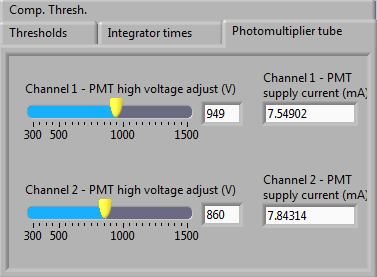
\includegraphics[scale=0.6]{PMT_instellen}
    \caption{In dit tab menu kan de spanning op de fotobuis worden ingesteld.
    Je kunt de slider verslepen of een spanning invoeren in het vakje.}
    \label{fig:PMT_instellen}
\end{figure}

\begin{figure}
    \centering
    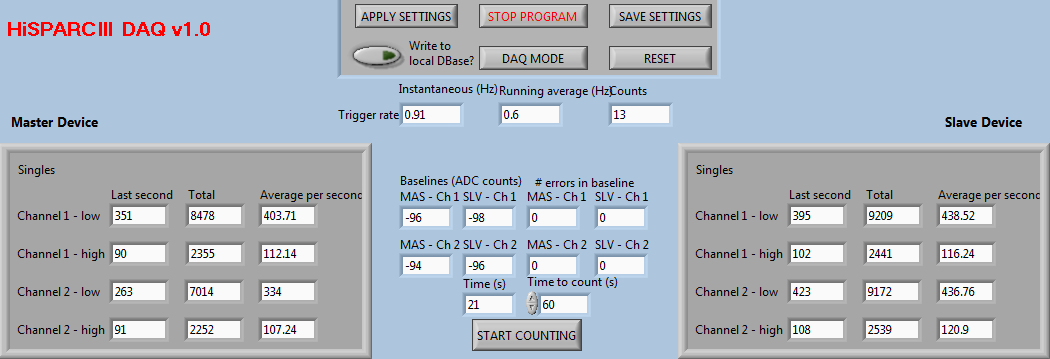
\includegraphics[scale=0.6]{instellen_PMT_values}
    \caption{In dit tab menu kun je op start counting drukken. De detectoren gaan dan meten.
    De waarden zouden voor de 3e kolom `average per second' bij `High' 120 moeten zijn en bij `low' ongeveer 250.
    Dit figuur heeft dus alleen voor detector 4 nu een goede waarde van 120.
    Daarom moet je de count ook de volledige 60 s laten lopen.}
    \label{fig:instellen_PMT_values}

\end{figure}

\end{document}
